\documentclass[12pt]{mythesis}

 % \makeglossaries
 % % \loadglsentries{glossaries_entries}
 % %%% A
 % %%% C
 % %%% D
 % %%% E
 % \newglossaryentry{EHV}{name=EHV, description={Extremely High Velocity}}
 % %%% F
 % \newglossaryentry{FoV}{name=FoV, description={Field-of-View}}
 % \newglossaryentry{FWHM}{name=FWHM, description={Full-Width Half-Maximum}}
 % %%% G
 % \newglossaryentry{GMCs}{name=GMCs, description={Giant Molecular Clouds}}
 % %%% H
 % \newglossaryentry{HST}{name=HST, description={Hubble Space Telescope}}
 % %%% I
 % \newglossaryentry{IHV}{name=IHV, description={Intermediate High Velocity}}
 % %%% K
 % %%% L
 % %%% M
 % %%% N
 % %%% O
 % %%% P
 % %%% Q
 % %%% R
 % \newglossaryentry{RA}{name=RA, description={Right Ascension}}
 % %%% S
 % \newglossaryentry{S/N}{name=S/N, description={signal-to-noise ratio}}
 % \newglossaryentry{SHV}{name=SHV, description={Standard High Velocity}}
 % %%% T
 % %%% U
 % %%% Y
 % \newglossaryentry{YSO}{name=YSO, description={Young Stellar Object}}
 % %%% Z


\title{Observing the Sun: From start to finish. }
\author{Pablo Santamarina Guerrero}
\date{\today}
\institution{%
 Instituto de Astrofísica de Andalucia (IAA-CSIC)\\
 \vspace{0.5cm}
 Programa de Doctorado en Física y Matemáticas (FisyMat)\\
 Universidad de Granada\\
}
\advisor{%
 {\large\bf Dr. David Orozco Suárez}\\
 \vspace{0.25cm}
 {\large\bf Dr. Julián Blanco Rodríguez}\\
}
\logo{%
  
\includegraphics[width=.47\linewidth]{images/LogosIAA_SO_Color.png}
  
\includegraphics[width=.47\linewidth]{images/UGR-MARCA-02-color.png}
}

\begin{document}
\frontmatter %Use lowercase Roman numerals for page numbers
\maketitle
%\restoregeometry
\cleardoublepage

\chapter*{Acknowledgements}
dkshfgsidgfisgdfisdfs
Agradecimientos

\chapter*{Resumen}

Resumen de la tesis

\chapter*{Summary}

Summary of the thesis

\tableofcontents

\mainmatter % Now Use Arabic numerals for page numbers
\chapter{Introduction}

\section{Motivation of our work}

\chapter{Designing and callibrating an instrument.}

\section{Spectropolarimeters: TuMag's design}
\section{Calibration of TuMag}

\chapter{Operation and data reduction.}

\section{TuMag's Observation modes and data reduction.}
\section{Challenges in data reduction: Etalon Cavity Map.}

\chapter{Scientific exploitation.}




\section{Persistent Homology in Solar Magnetograms.}

\subsection{Persistent Homology}

Persistent homology stands out as a prominent technique within the topological data analysis toolkit, primarily for its capacity to capture the shape and distribution information of a dataset. The algorithm is rooted in the mathematical framework of homology groups. In topology, these groups measure the number of $n$-dimensional holes in a data set, or in other words, the number of connected components for a  $0^{th}$ dimensional analysis, holes or rings for a $1^{st}$ dimensional analysis, spherical voids for the $2^{nd}$ dimensional analysis, and so on. 

The primary objective of persistent homology is not only to compute the homology groups of a given dataset but also to study how they vary at different scales. To achieve this, the input data undergoes a process of division into a series of sequential subspaces, with each subspace encompassing the previous one. This sequential process, known as filtration, begins with a starting subspace comprising a single point from the original dataset. Subsequent subspaces are then constructed by incrementally adding points to the previous subspace until the final subspace includes all points of the original dataset. 

After the filtration process is performed, persistent homology algorithms shift their focus to analyzing the evolution of topological features across the different subspaces. Specifically, they record the filtration value at which a new feature appears, meaning that it is absent in the previous subspace, and when it disappears, meaning that it is no longer present in the following subspaces. These two events are known as the birth and death of a topological feature, respectively. 

In a nutshell, the $n$-dimensional persistent homology of a dataset with a given filtration can be described as the aggregation of all n-dimensional features (homology groups) that were created (birth) and subsequently eliminated (death) during the filtration process \citep{ph_filtration}.

When applying persistent homology on a greyscale image, our focus lies in filtering the data according to the pixel values. Multiple filtering approaches exist, with the most extended ones being sublevel and superlevel filtrations, both based on the concept of thresholding. In these filtrations, the image is cropped to a specific value, forming a subspace that includes all pixels with values higher than this value in a superlevel filtration, or lower in a sublevel filtration. This cropping value (i.e. the filtration value) is systematically varied from the lowest to the highest values of the image, or vice versa, thus generating a different subspace for each value. As a result, the persistence homology analysis captures and examines the evolution of topological features across different thresholds, enabling insights into the image's structural properties at various scales \citep{ph_image_filtration}.

hsidihfd
dlfjhdglh
kfhgf


A more formal way of defining these filtrations can be done by considering an image as a discrete representation of a function $f$, defined over a two-dimensional space $\mathbb{X}$, such that: 
\begin{equation}
    f :  \mathbb{X} \longrightarrow  \mathbb{R} \ \ .
\end{equation}
Let $\mathbb{S} _\phi$ be the subspace of $\mathbb{X}$ for a filtration value of $\phi$. In such a case, a filtration can be expressed as:
\begin{equation}
    \mathbb{X}: \mathbb{S}_{\phi_0} \subset \mathbb{S}_{\phi_1} \subset \mathbb{S}_{\phi_2}\subset... \subset \mathbb{X}\ \ .
\end{equation}
With this formulation, a topological feature with birth-death coordinates:
\begin{equation}
(B, D) = (\phi_ I, \phi _ {II}) \ \ ,
\end{equation} 
corresponds to a feature that appears for the first time during the filtration process at the subspace $\mathbb{S}_{\phi _ I}$, and \textit{persists} until the subspace $\mathbb{S}_{\phi _ {II}}$, where it ceases to exist.

In a sublevel filtration, each subspace can be expressed as:
\begin{equation}
    \mathbb{S} _ \phi = f ^{-1} \left( ( -\infty, \phi ] \right) \ \ ,
    \label{eq: sublevel}
\end{equation}
where $\phi_0$ is selected as the lowest value for any given pixel and its value is increased until the subspace includes all pixels. On the contrary, in a superlevel filtration, the subspaces can be expressed as:
\begin{equation}
    \mathbb{S} _ \phi = f ^{-1} \left( [ \phi, \infty ) \right)\ \ , 
    \label{eq : superlevel}
\end{equation}
where $\phi_0$ is selected as the highest value for any given pixel and its value is decreased along the filtration.

Various methods exist for representing the information derived from a persistent homology analysis, including Betti numbers, persistence bars, and persistent diagrams (PDs) (\citealt{pd_stability}, \citealt{pbars}), among many others. For this study, we will utilize the PDs as our chosen approach due to their straightforward interpretation and extended use. A $n$-dimensional PD is a multiset of Birth-Death pairs, ($B _ i, D _ j$), with multiplicity $k$, where each pair measures the number ($k$) of $n$-dimensional components that have been born at the filtration subspace $\mathbb{X}_i$ and died in $\mathbb{X}_j$, that is usually represented in a 2D scatter plot. 


\begin{figure}
    \centering
     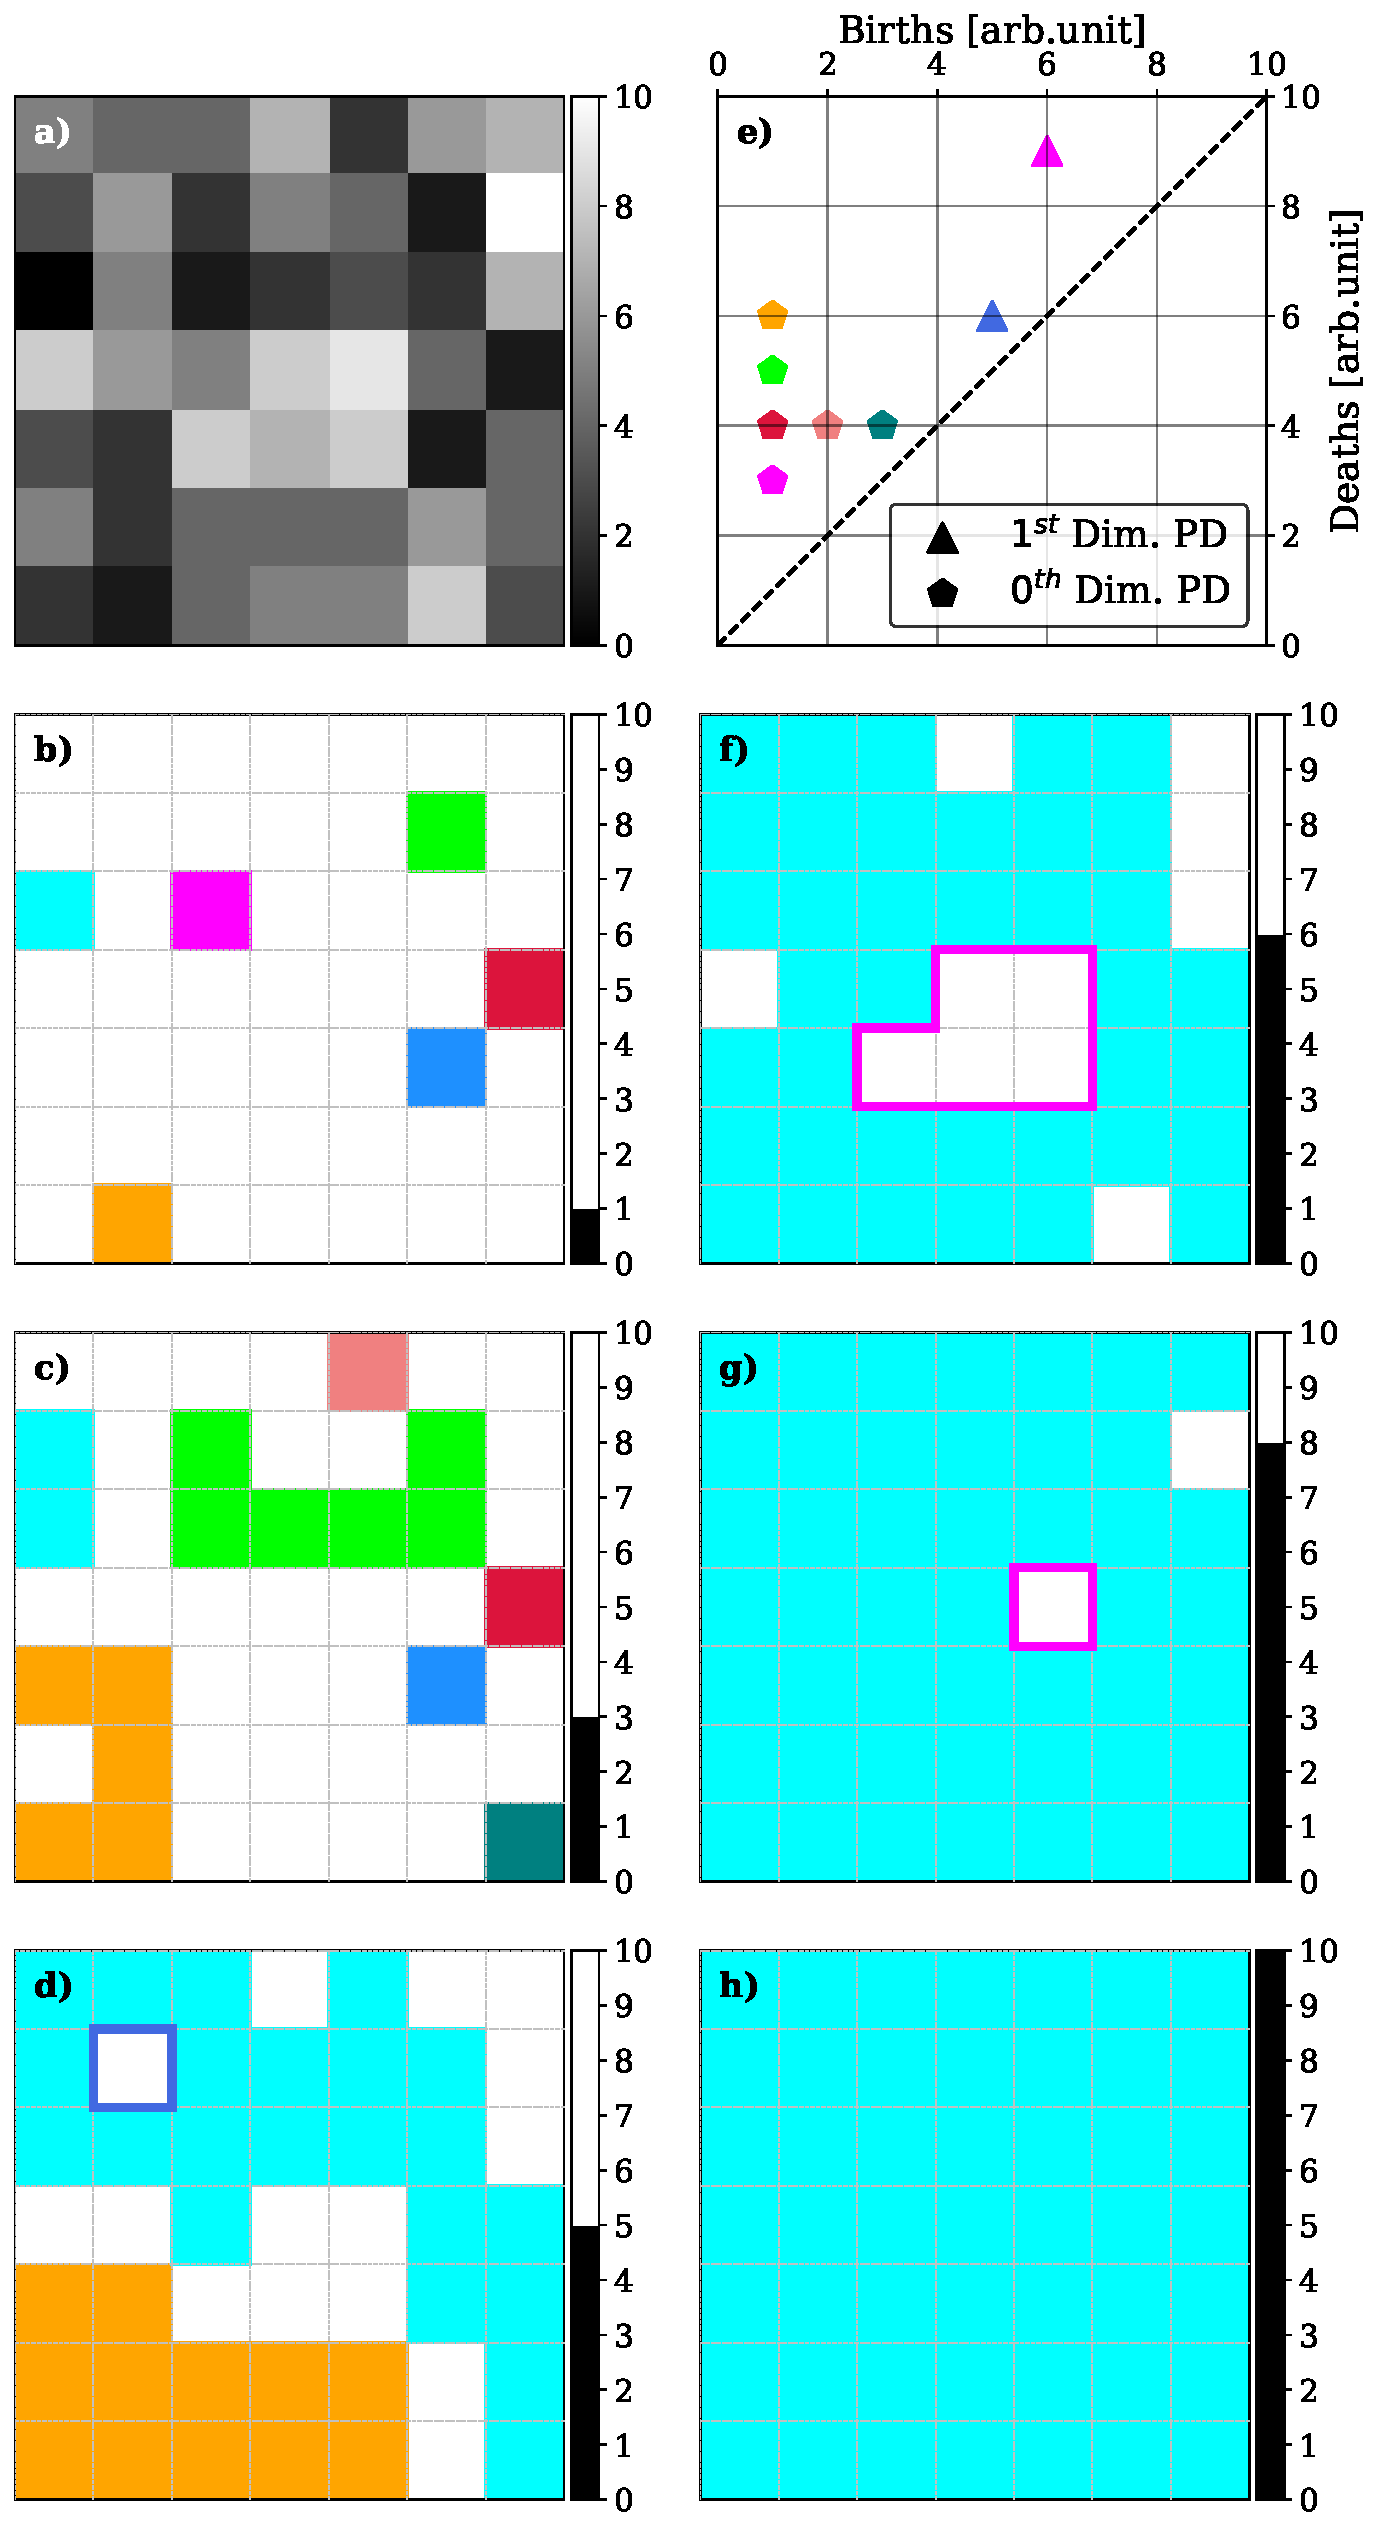
\includegraphics[width=8cm]{figures/PersistentHomology/ImageFiltering_example.pdf}
    \caption{Sublevel filtration of a greyscale image and PDs of the $0^{th}$ and $1^{st}$ dimensions. Panel a) shows the input data. In panels b), c), d), f), g), and h) different snapshots of the filtration process are shown. The value of the filtration parameter, $\phi$ is shown in the color bar at the right of each image. Only pixels with a value lower than the filtration value (colored pixels) belong to the subspace shown in each snapshot. Different homology groups are represented with different colors at each snapshot. For connected components ($0^{th}$ dimensional homology groups) the whole pixel is shown with the corresponding color. For rings, ($1^{st}$ dimensional homology groups), only the border of each hole is colored. In panel e) the PDs of both dimensions are shown. The color of each point in the diagram is the same as the one used to plot the corresponding topological feature in other panels. An animation depicting the whole filtration process is also provided as part of the article.}
   \label{fig_ph: Image Filtration Example}
\end{figure}


The process of generating a PD of a greyscale image is as follows. We start by selecting the filtration direction (sublevel or superlevel) and the dimension of the analysis (either 0 or 1). We initialize a threshold as the highest or lowest value from the image, depending on the choice of filtration. We then perform the filtration by systematically adjusting the threshold and creating a binary image for each threshold. This process divides the image into two sets: pixels with values above the threshold and pixels with values below it. The choice of filtering determines which of the two sets makes up the subspace. We then look for the existing topological features within each of these subdivisions. The specific process by which these features are identified is detailed in the next paragraph, where the structures corresponding to both dimensions are illustrated using the example shown in Fig.~\ref{fig_ph: Image Filtration Example}. We repeat this process until the threshold reaches the opposite limit to that from which it started. Along this process, we follow the appearance, merging, and disappearance of connected components. When two components merge, the longer-lived one (\textit{i.e}. the first to appear along the filtration process) absorbs the younger one, thus resulting in the death of the second \citep{eldest}. We determine the birth and death for each component based on the thresholds at which these events occur.  Finally, we construct a scatter plot where the horizontal axis represents the birth values and the vertical axis represents the death values. Each point on this plot corresponds to a persistence point, whose coordinates reveal the scales at which the corresponding topological feature is present.

An example of this process with a sublevel filtration is shown in Fig.~\ref{fig_ph: Image Filtration Example}. Panel a) displays the input data, panels b), c), d), f), g), and h) show some of the key steps of the filtration process, and, lastly, panel e) displays the PD for a $0^{th}$ and $1^{st}$ dimensional analyses. These plots illustrate how connected components and rings are born and then die as we increase the filtration level. As these components (shown in different colors) increase in size and come into contact with other components, one absorbs the other, thus resulting in the death of the second. This phenomenon is shown in panels b) to d), where we observe the progression of the components until only the blue and orange connected components remain. Additionally, the diagrams also reveal the appearance of two rings in the data (panels f) and g)). These rings are found when pixels that do not belong to the subspace are surrounded by a connected component, and die when those pixels are included in the component as the threshold increases (blue ring in panel f)). Finally, the PD (panel e)) displays the birth and death values (i.e. the filtration value) of all the features, of dimensions 0 and 1, that have been identified (birth) and subsequently eliminated (death) throughout the filtration process. 

\subsection{Persistent Images}

The PD displayed in Fig.~\ref{fig_ph: Image Filtration Example} contains only a limited number of points due to the simplicity of the input image. However, when analyzing real data, these diagrams can consist of hundreds or even thousands of birth-death pairs with high multiplicities, simply due to the size of the images. Additionally, features not only representing the genuine behavior of the data but also reflecting the distribution of noise appear on the diagrams. To address this complexity, several strategies have been developed to simplify the information from PDs, such as persistence curves  \citep{persistence_curves}, persistence landscapes \citep{persistence_landscapes}, or persistence images (PI) \citep{persistence_images}. In this study, we will focus on the latter, due to its noise filtering capabilities and because the representation of the results remains in a Birth-Death diagram, allowing for easy interpretation of the results, similar to a persistence diagram.

PIs are a condensed form of a persistence diagram, offering a concise and easy-to-understand representation of its topological features.  They capture the spatial distribution and persistence information of these features, allowing for the enhancement of the most relevant ones and filtering of the others. A PI is constructed using the concept of persistence. Each topological feature, represented by a point in a PD, has a persistence, $\pi$, of:

\begin{equation}
    \pi = D - B
    \label{eq: persistence}
\end{equation}


where $(B, D)$ are the corresponding birth-death coordinates in the diagram. A feature with a large persistence is present at different scales in the data and therefore is more likely to represent the real behavior of the data. On the contrary, short-lived features are typically associated with the noise distribution and usually do not provide much information about the data.

\begin{figure}
    \centering
    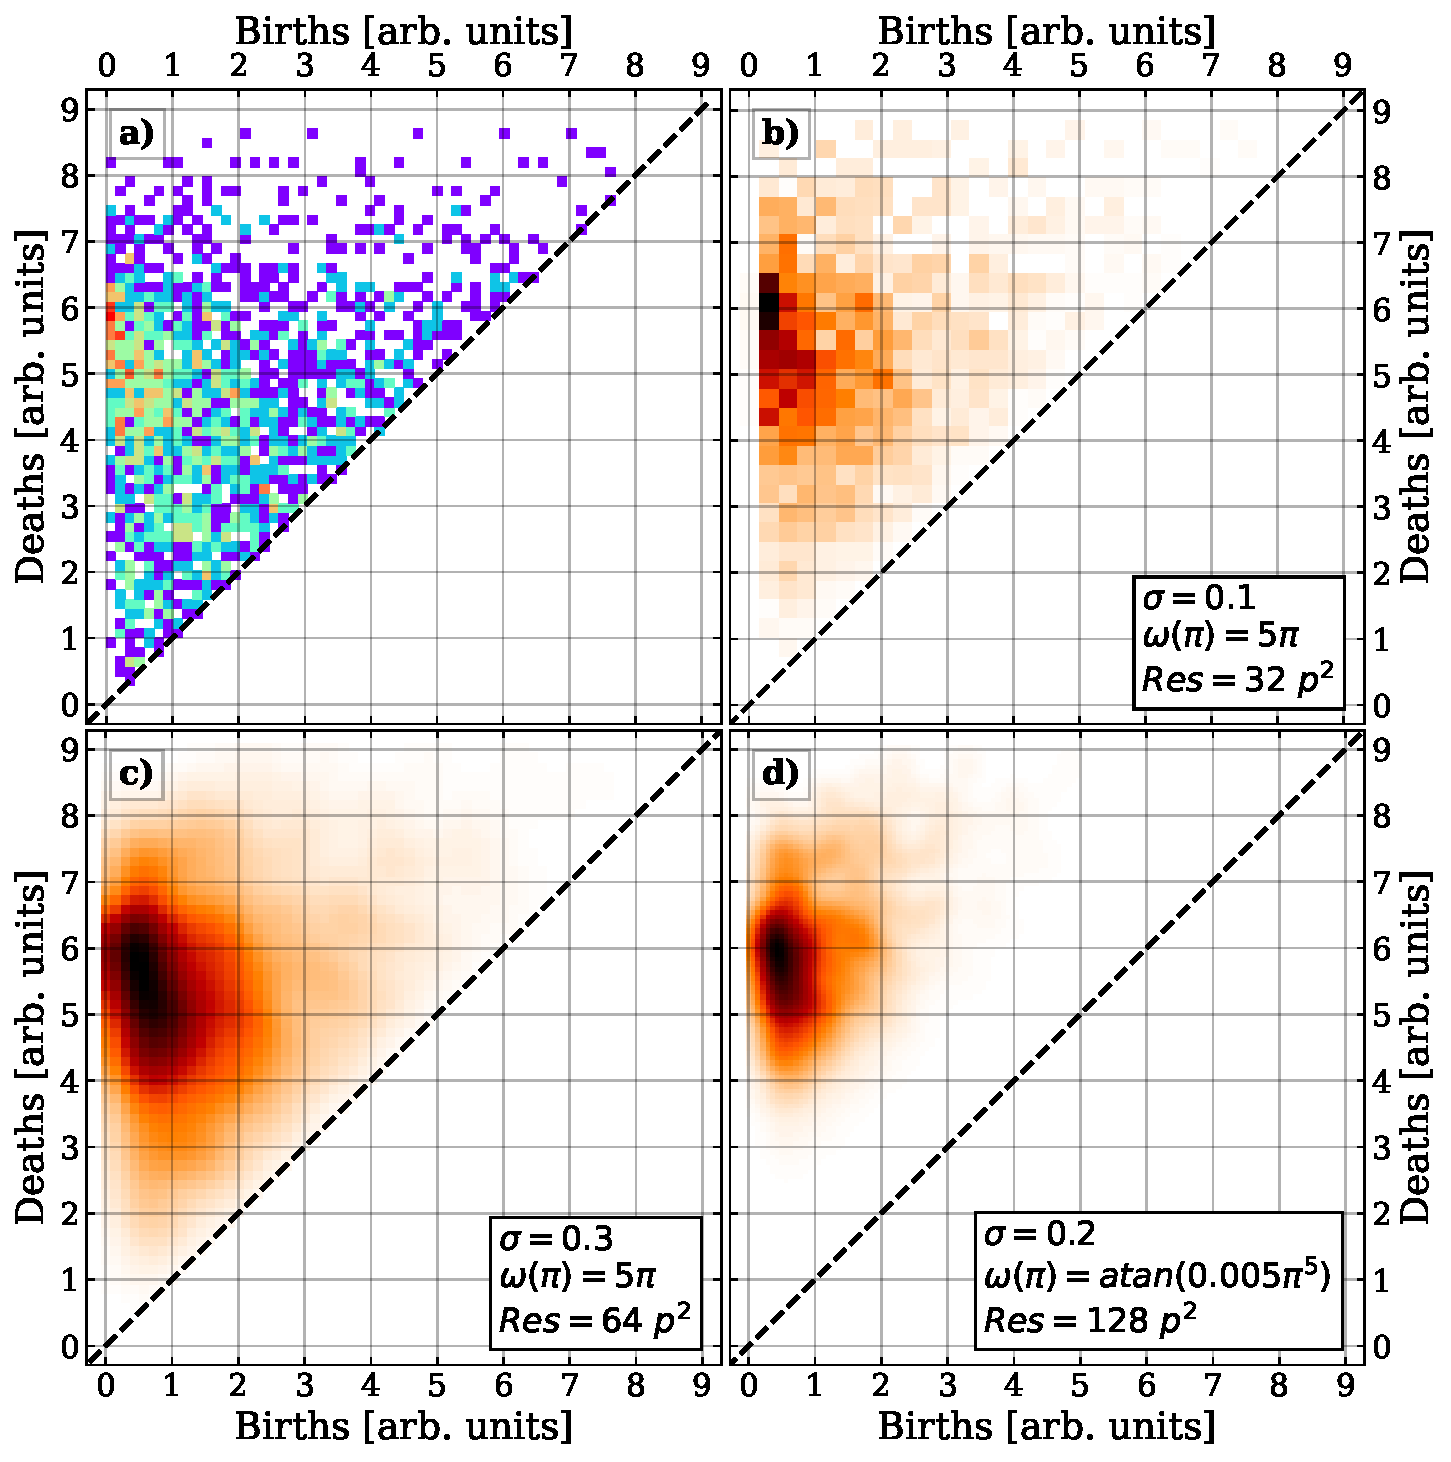
\includegraphics[width=12cm]{figures/PersistentHomology/PI_Example.pdf}
    \caption{Panel a) shows an example of a persistence diagram as a 2D histogram. The color of each bin represents its multiplicity, with the red spots corresponding to higher values. Panels b), c), and d) show three different examples of PIs. The three parameters given in the legends of the PIs are: the standard deviation ($\sigma$) of the Gaussian kernel ($K (z)$), the weighting function, and the resolution of the image PI in pixels (p).}
   \label{fig_ph: PI Example}
\end{figure}

When constructing a PI, a weighting function, $\omega (\pi)$, is employed to assign weights to each point in the diagram, ensuring that longer-lived features have greater weights than shorter-lived ones. There are multiple choices for the shape of the weighting function, which are entirely dependent on the aims of the study and data type. The simplest example is often a linear or power-law relation ($\omega (\pi) = a \pi ^b$), where $a$ and $b$ can be tuned to assign progressively higher weights to higher persistencies, thus focusing the study on the longer-lived components. On the other hand, if the objective is to filter out noise while assigning similar weights to all non-noise points so that all points have a similar relevance in the analysis, the chosen function is usually an arc-tangent.

The PI is then generated by dividing the persistence diagram plane into a grid with a desired resolution. Within each grid region (or pixel), the weighted features of the diagram within the region are added up using a kernel density estimation. The kernel function, $K (z)$, can be tuned to suit the nature and objectives of the analysis, with Gaussian functions being the most common approach. 

The resultant PI is a 2D matrix, wherein each pixel corresponds to a specific area in the persistence diagram, and its value represents the cumulative weight of the topological features found within that area. In Figure \ref{fig_ph: PI Example}, three examples of PI (panels b), c), and d)) are presented for the same persistence diagram (panel a)), where distinct choices of resolution, kernel function, and weighting function have been applied to each image.




All the PDs, PIs, and the rest of the analysis tools presented in this work, have been computed using the Homcloud python package \citep{homcloud}.


\subsection{Data}

In this work, we study the results of applying persistent homology to different regimes of solar activity by applying the analysis to both quiet Sun and active region magnetograms.

\subsubsection{Quiet Sun observations}

The study of quiet Sun regions requires high magnetic spatial and temporal resolutions and sensitivities to be able to capture the small-scale evolution of the magnetic structures due to their weak signals ans short time scales \citep{quiet_sun_living_review}. For this reason, we employ observations taken by the Solar Optical Telescope (SOT; \citealt{sot}) aboard the \textit{Hinode} satellite \citep{Hinode}, a space-borne solar observatory. In particular, we employ observations from Hinode's Operation Plan (HOP) 151. These observations consist of long ($\ge 20$ h) and mostly uninterrupted sequences of measurements of the Narrowband Filter Imager of the Na I D1 line at 5896 \r{A} taken with a cadence of $50-70$ s. The data correction of the selected observation sets has been carried out in \citep{gosic}.


\subsubsection{Active regions observations}

We employ observations of active regions (ARs) taken by the Helioseismic and Magnetic Imager (HMI; \citealt{hmi1}, \citealt{hmi2}) on board the Solar Dynamics Observatory \citep{SDO}. HMI provides a continuous observation of the Sun where a full-disk magnetogram, as well as Dopplergrams, are provided at all times. The full-disk, uninterrupted observations of HMI make it a very suitable instrument to study the evolution of active regions as the formation and development of active regions can be fully captured. 

We focus the analysis on a series of newly-emerging ARs identified in \citep{toriumi}. In particular, we employed the 12-minute cadence observations taken during the period from May 2010 to June 2011, which corresponded to a period of low solar activity.

\subsubsection{Analysis and results}

\begin{figure}
    \centering
     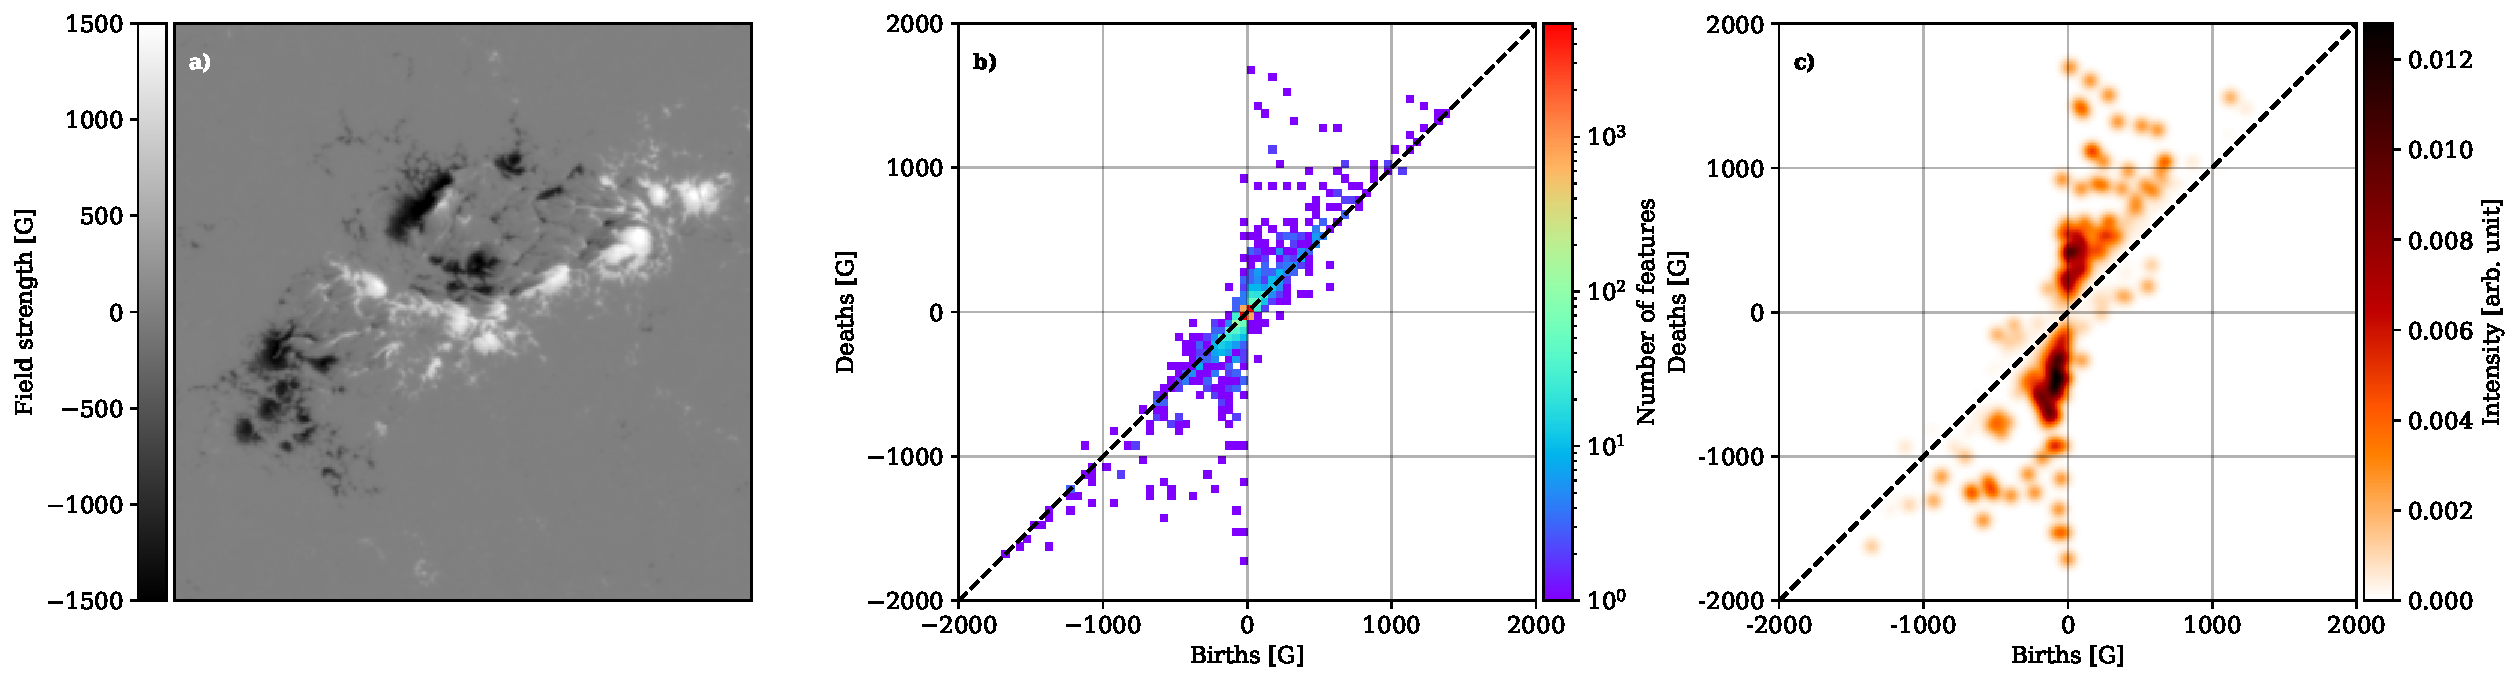
\includegraphics[width=8cm]{Figures/PersistentHomology/PI_PD_example.pdf}
    \caption{(a) SDO/HMI magnetogram taken on 2011-02-13 depicting an active region (NOAA AR 11158). (b) The corresponding PD combining superlevel and sublevel filtrations. (c) PI generated from the PD in panel b) with the following configuration: Resolution =  1000 pixels$^2$ ($4\ G$ per pixel), weighting function: $\omega (\pi) = \arctan (5\times 10 ^{-8} \pi ^{3})$ and a gaussian kernel with $\sigma = 40\ G$.}
   \label{fig: PD+PI_example}
\end{figure}


The application of persistent homology to a specific dataset can vary depending on the aims of the study. Different dimensions of the analysis and various types of filtrations focus on distinct features within the data. It is crucial to have prior knowledge of the expected structures and relevant features to be captured in the analysis in order to determine the appropriate approach. In this section, we aim to outline the most appropriate approach for studying the particular case of solar magnetograms.

The solar magnetograms employed here represent the longitudinal component of the magnetic field on the photosphere and are typically presented as greyscale images, as shown in Figure \ref{fig: PD+PI_example}, panel a). The polarity of the line-of-sight magnetic field is indicated by the sign of each pixel, where positive and negative signals correspond to field lines pointing towards and away from the observer. Applying a single filtration to a greyscale image only displays features corresponding to one polarity (positive or negative) in a PD. However, to conduct a comprehensive study of the magnetic field, both polarities are essential, thus necessitating the use of two separate filtrations with different filtration directions.

\begin{figure}
    \centering
     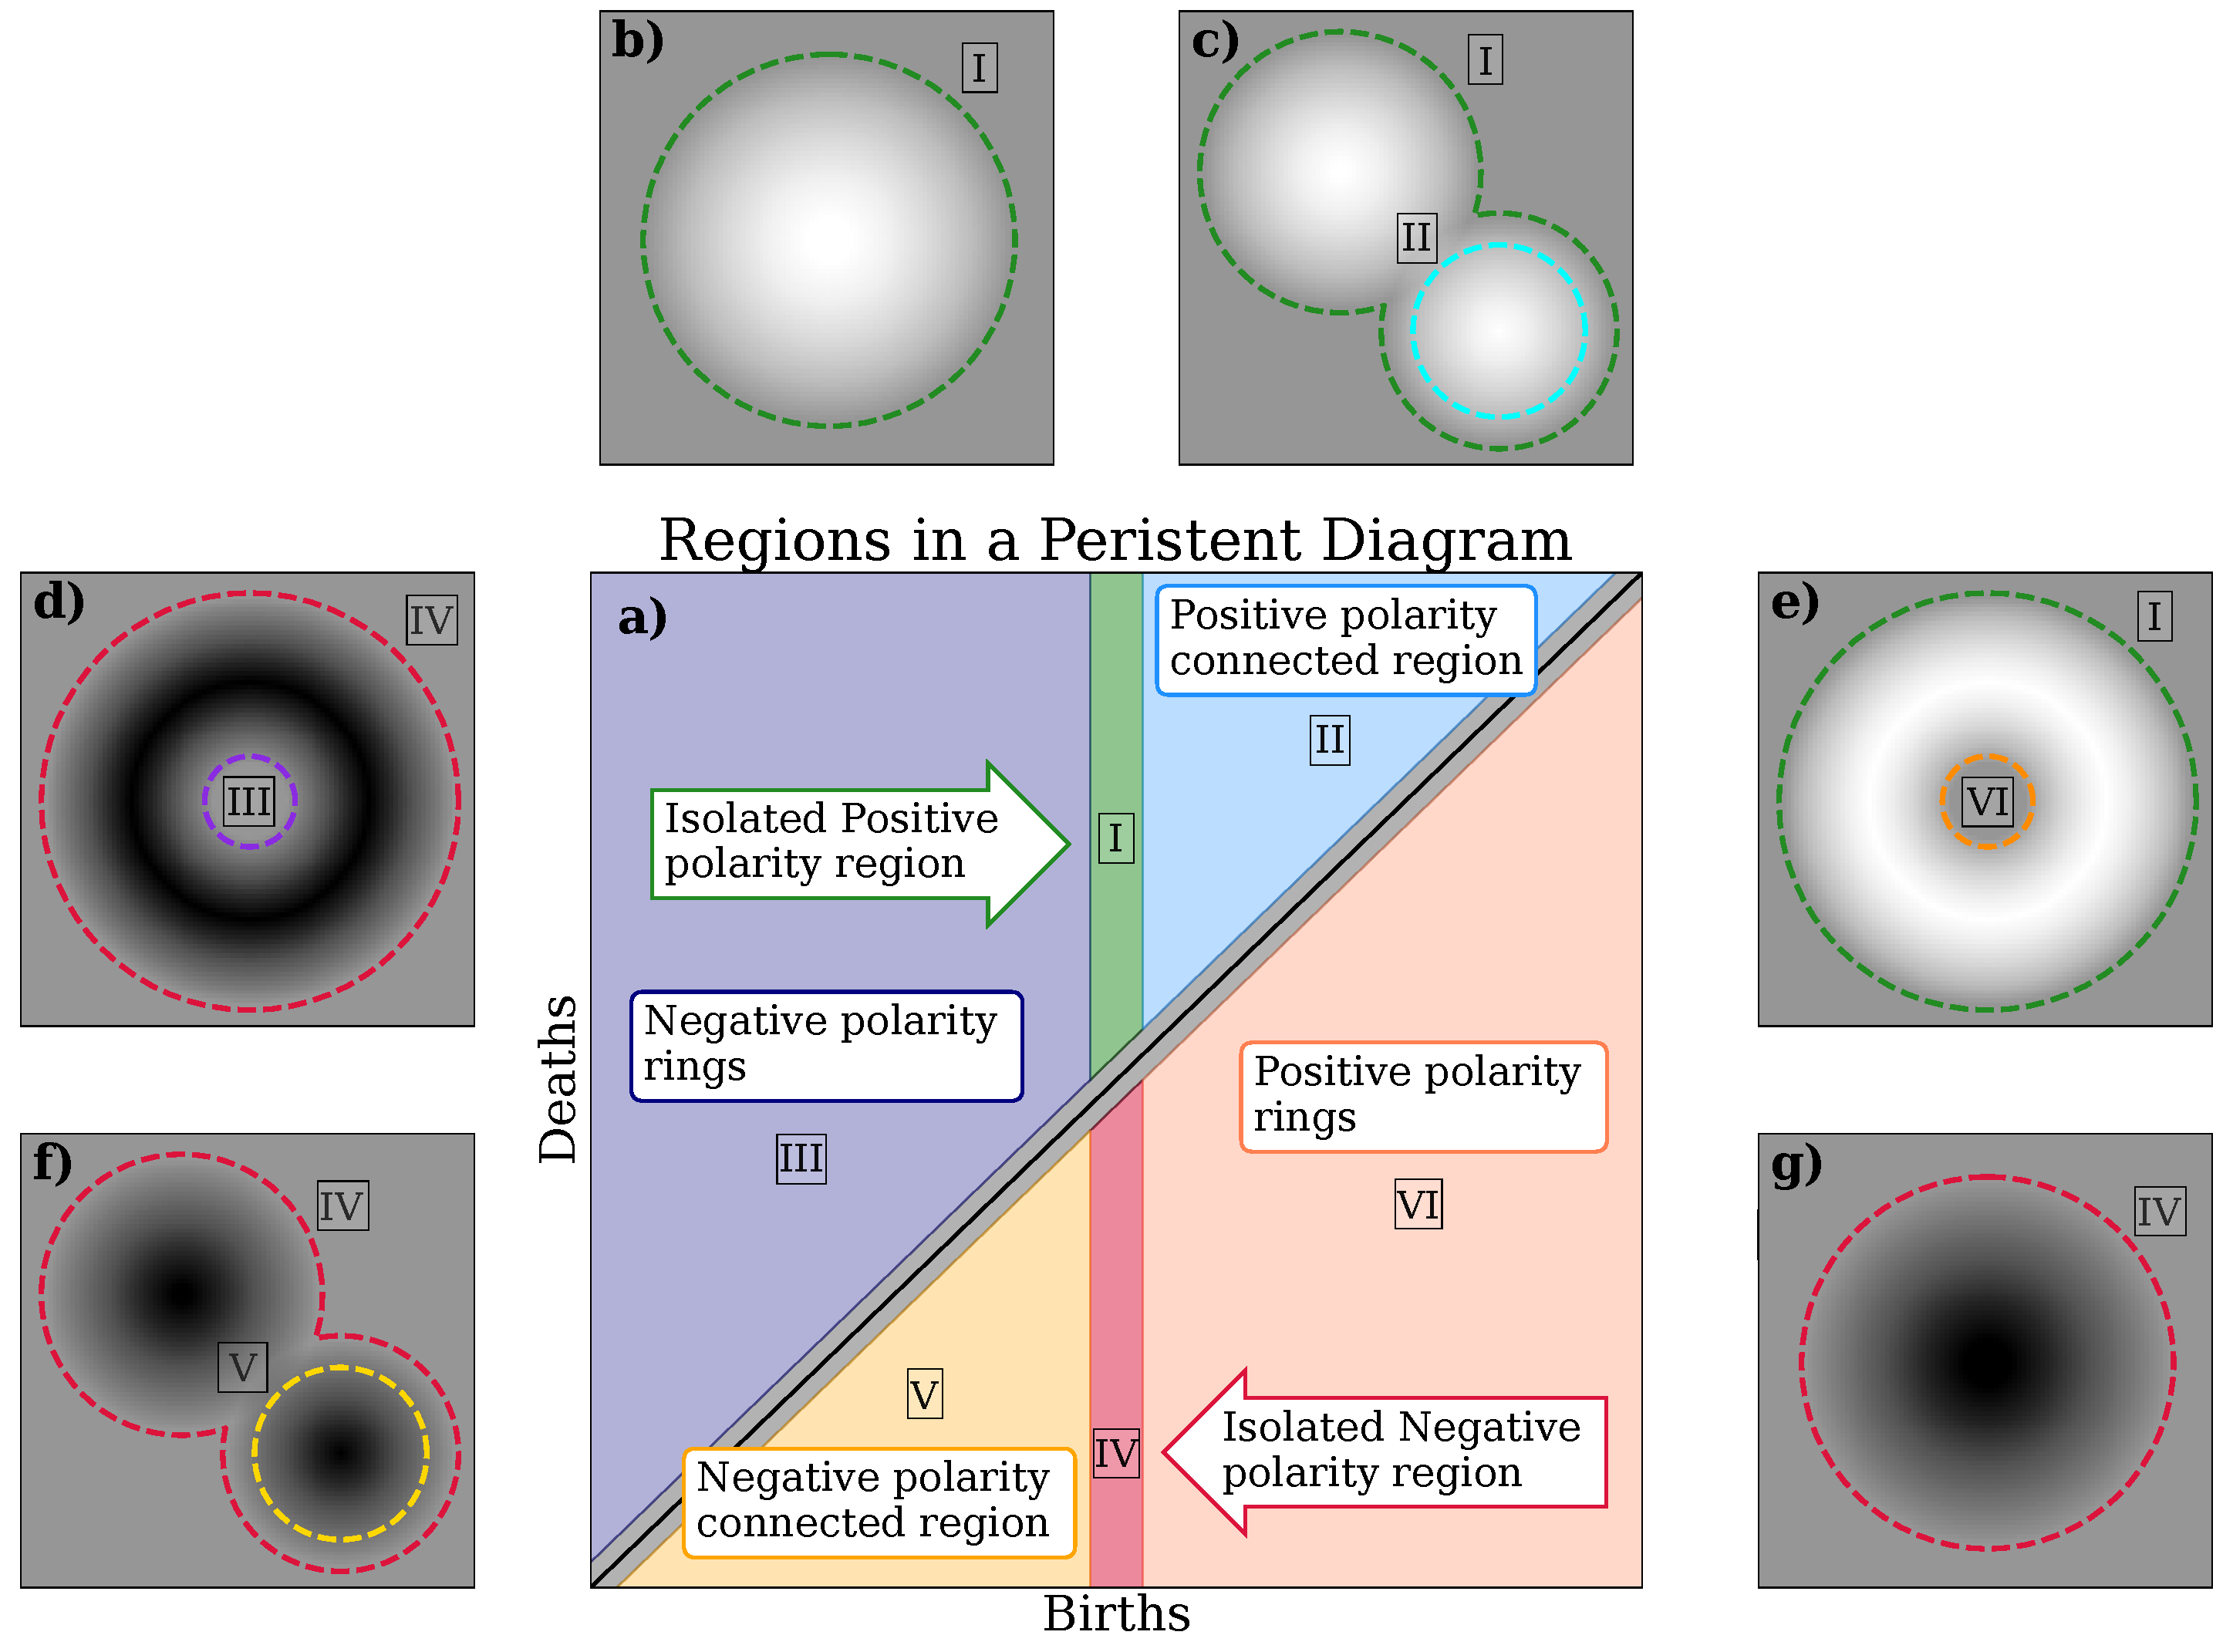
\includegraphics[width=8cm]{Figures/PersistentHomology/Regions_anotated.pdf}
    \caption{Schematic representation of the PD and the different regions (panel a)). The magnetic structures corresponding to the topological features found in the different regions are shown in panels b) to g), with each feature identified by a ring with the corresponding color.}
   \label{fig: PD REGIONS}
\end{figure}

We determined that a combination of superlevel and sublevel filtrations with a $1^{st}$-dimensional persistent homology analysis was the most suitable approach for studying solar magnetograms. This choice is based on two main reasons. Firstly, the $1^{st}$ dimensional analysis allows us to identify the most prominent features in a PD, which is not the case in the $0^{th}$ dimensional analysis where the strongest feature does not appear in the diagram as it never dies (see Fig.~\ref{fig: PD Example Images}). Secondly, by combining superlevel and sublevel filtrations, we can display the results of both filtrations in a single diagram. Features corresponding to different filtrations will have persistencies with opposite signs (features found in a superlevel filtration will be born at higher filtration values than their death, resulting in a negative lifespan). This enables us to construct a PD in which all features displayed above the identity line (with positive persistencies) correspond to the sublevel filtration, and those below the line correspond to the superlevel filtration (see panel b) in Fig.~\ref{fig: PD+PI_example}).

The PDs, and consequently the PIs, offer valuable insights into the magnetic structures present in the magnetograms. The location of a topological feature on the diagram is completely determined by the properties of the corresponding magnetic structure. Specifically, this position is influenced by factors such as the maximum intensity of the magnetic field, its proximity to other magnetic structures, and its geometric shape, including the presence of holes or pores within the structure. These characteristics allow us to partition the diagram into distinct regions, where topological features within each region correspond to different types of magnetic structures.


We distinguished between six distinct regions in the diagram. Figure \ref{fig: PD REGIONS} illustrates these regions in panel a) and provides schematic representations of the corresponding magnetic structures in panels b) to g). The regions are as follows: first, topological features located above the identity line (positive persistencies) with birth values close to 0 (region I in the diagram). Features within this region represent isolated magnetic structures of positive polarity, that is, patches of positive magnetic flux fully enclosed by an absence of any magnetic field. The threshold defining what is considered ``close to 0$"$ is determined by the data's properties. To identify isolated structures, we set the threshold as a function of the statistical properties of the background signal (i.e. areas of the magnetogram with little magnetic flux). Specifically, the limits for this region are set as $(-5 \sigma _ {bg}, 5 \sigma _ {bg})$, where $\sigma _ {bg}$ denotes the standard deviation of the background signal found in a $15\times 15$ pixels box devoid of strong magnetic structures.

The second region (II in the diagram) comprises features above the identity line with positive birth values, representing connected structures with positive polarities, that is, positive magnetic field structures in contact with another positive structure but not fully merged. The third region (region III) contains topological features above the identity line with negative birth values, which corresponds to magnetic structures of negative polarity exhibiting a ring-like attribute, namely, structures with pores or holes. These three regions of the diagram have counterparts with negative persistencies. Thus, features associated with isolated structures of negative polarities are found in the region with a birth value close to 0 but below the identity line (region IV), features for connected negative structures are also located below the line but with negative birth values (region V). Lastly, features arising from positive magnetic structures with ring-like attributes are found below the identity line but with positive birth values (region VI).


\chapter{Summary and conclusions}

The conclusions are \dots

\appendix

\chapter{Profile derivatvies}

\citep{hale}
\bibliography{bibliography}

\cleardoublepage
\layout

\end{document}
